%%
% This is an Overleaf template for presentations
% using the TUM Corporate Desing https://www.tum.de/cd
%
% For further details on how to use the template, take a look at our
% GitLab repository and browse through our test documents
% https://gitlab.lrz.de/latex4ei/tum-templates.
%
% The tumbeamer class is based on the beamer class.
% If you need further customization please consult the beamer class guide
% https://ctan.org/pkg/beamer.
% Additional class options are passed down to the base class.
%
% If you encounter any bugs or undesired behaviour, please raise an issue
% in our GitLab repository
% https://gitlab.lrz.de/latex4ei/tum-templates/issues
% and provide a description and minimal working example of your problem.
%%

%\PassOptionsToClass{onlytextwidth}{beamer}

\documentclass[
  german,            % define the document language (english, german)
  aspectratio=169,    % define the aspect ratio (169, 43)
  % handout=2on1,       % create handout with multiple slides (2on1, 4on1)
  % partpage=false,     % insert page at beginning of parts (true, false)
  % sectionpage=true,   % insert page at beginning of sections (true, false)
]{tumbeamer}


% load additional packages
\usepackage{booktabs}
\usepackage{graphicx}
\usepackage{tikz}
\usepackage{url}
\usepackage{pgf}
\usepackage{pgfplots}
\usepackage{hyperref}
\usepackage{pmboxdraw}
\usepackage{float}
\usepackage{babel}[ngerman]
\usepackage{csquotes}[autostyle]
\usepackage[useregional]{datetime2}
\usepackage[cache=true]{minted}
\usemintedstyle{borland}
\usepackage{listings}

% tikz
\usetikzlibrary{patterns}
\usetikzlibrary{positioning}
\usetikzlibrary{overlay-beamer-styles}

% minted
\setminted{
    fontsize=\small, 
    frame=none,
    breaklines=true,
}

% image path
\graphicspath{ {./resources/} }

% presentation metadata
\title{Übung 04: Rekursion und Calling Convention}
\subtitle{Einführung in die Rechnerarchitektur}
\author{Niklas Ladurner}

\institute{\theChairName\\\theDepartmentName\\\theUniversityName}
\date{\DTMdisplaydate{2024}{11}{8}{-1}}

\footline{\insertauthor~|~\insertshorttitle~|~\insertshortdate}


% macro to configure the style of the presentation
\TUMbeamersetup{
  title page = TUM tower,         % style of the title page
  part page = TUM toc,            % style of part pages
  section page = TUM toc,         % style of section pages
  content page = TUM more space,  % style of normal content pages
  tower scale = 1.0,              % scaling factor of TUM tower (if used)
  headline = TUM threeliner,      % which variation of headline to use
  footline = TUM default,         % which variation of footline to use
  % configure on which pages headlines and footlines should be printed
  headline on = {title page},
  footline on = {every page, title page=false},
}

% available frame styles for title page, part page, and section page:
% TUM default, TUM tower, TUM centered,
% TUM blue default, TUM blue tower, TUM blue centered,
% TUM shaded default, TUM shaded tower, TUM shaded centered,
% TUM flags
%
% additional frame styles for part page and section page:
% TUM toc
%
% available frame styles for content pages:
% TUM default, TUM more space
%
% available headline options:
% TUM empty, TUM oneliner, TUM twoliner, TUM threeliner, TUM logothreeliner
%
% available footline options:
% TUM empty, TUM default, TUM infoline


\begin{document}

\maketitle

\begin{frame}[c, fragile]{}{}
  \begin{center}
    \LARGE  Keine Garantie für die Richtigkeit der Tutorfolien.

    \Large Bei Unklarheiten/Unstimmigkeiten haben VL/ZÜ-Folien recht!
  \end{center}
\end{frame}

\begin{frame}[c, fragile]{Caller vs. Callee}{}
  \begin{columns}[c]
    \begin{column}{0.5\textwidth}
      \begin{minted}[fontsize=\scriptsize]{gas}
caller:
# aufrufende Funktion (Caller)

# Wir speichern die Rücksprungadresse auf 
# den Stack -> ra ist Caller-saved!
addi sp, sp, -16
sw ra, 0(sp)

# ... irgendwas, was t0 verwendet

# da t0 caller-saved ist, müssen wir uns
# t0 absichern, wenn wir den Inhalt später
# noch brauchen
sw t0, 4(sp)
# ...
jal ra, callee  # Sprung zur Unterfunktion
# ...
lw t0, 4(sp)
# ... wieder irgendwas mit t0
lw ra, 0(sp)
        \end{minted}
    \end{column}
    \begin{column}{0.5\textwidth}
      \begin{minted}[fontsize=\scriptsize]{gas}
addi sp, sp, 16
jalr zero, 0(ra)

callee:
# aufgerufene Funktion (Callee)

# hier dürfen wir t0-t6 bspw. verändern
# falls wir s0-s6 verändern wollen würden,
# würden wir das so machen:
addi sp, sp, -16
sw s2, 0(sp)
sw s3, 4(sp)

# s2, s3 können jetzt verwendet werden!

lw s2, 0(sp)
lw s3, 4(sp)
addi sp, sp, 16
jalr zero, 0(ra)
      \end{minted}
    \end{column}
  \end{columns}
  \begin{center}
    \small{fürs Selbststudium :)}
  \end{center}
\end{frame}

\begin{frame}[c, fragile]{Caller- und Callee-saved Register}{}
  \begin{figure}[h]
    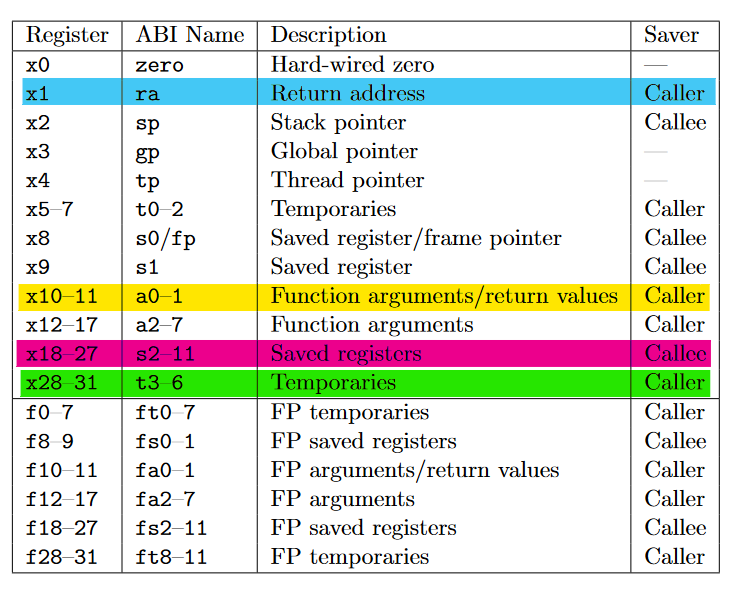
\includegraphics[height=0.75\textheight]{resources/w03_calling_conv_regs.png}
    \caption{Übersicht über die RISC-V-Register}
  \end{figure}
\end{frame}

\begin{frame}[c, fragile]{Calling Convention}{}
  \begin{itemize}
    \item \enquote{Aufrufkonvention} $\rightarrow$ lediglich eine Vereinbarung
    \item definiert Parameterüberabe, Rückgabe, Registersicherung, Stack etc.
    \item Datentypen $\le$ 4 Byte in a-Register, signextension
    \item Datentypen = 8 Byte in 2 a-Register, niedrigwertige Hälfte zuerst
    \item Datentypen > 8 Byte als Pointer (Zeiger auf Speicher)
    \item Falls zu wenige Register: Übergabe über Stack
    \item Stackpointer muss immer Vielfaches von 16 Byte sein!
  \end{itemize}
\end{frame}

\begin{frame}[c, fragile]{Rekursion}{}
  \begin{itemize}
    \item Funktion die \textbf{sich selbst aufruft}
    \item $\exists$ äquivalente iterative Funktion für jede rekursive Funktion
    \item Aufbau:
          \begin{enumerate}
            \item Abbruchbedingung(en)
            \item Sicherung von \verb|ra| und evtl. Parametern
            \item Vorbereitung der Parameter für den rekursiven Aufruf
            \item Rekursiver Aufruf
            \item Ergebnis des Aufrufs verwerten
            \item Wiederherstellung von \verb|ra|, \verb|sp|
            \item Rücksprung
          \end{enumerate}
  \end{itemize}
\end{frame}

\begin{frame}[c, fragile]{Rekursion: Beispiel}{}
  \begin{columns}[c]
    \begin{column}{0.4\linewidth}
      \begin{lstlisting}[
        basicstyle=\ttfamily,
        numbers=left,
        stepnumber=1,
        showstringspaces=false,
        tabsize=4,
        breaklines=true,
        breakatwhitespace=false,
        frame=single,
      ]
fun:
  addi sp, sp, -8
  sw ra, 0(sp)
  sw a0, 4(sp)
  beq a0, zero, end
  addi a0, a0, -1
  jal fun
  end:
  lw ra, 0(sp)
  addi sp, sp, 8
  jalr zero, 0(ra)
      \end{lstlisting}
      \small \textbf{Achtung}: 8 Byte nicht CC-konform, nur zur besseren Darstellung
    \end{column}
    \begin{column}{0.5\linewidth}
      \begin{enumerate}
        \item Abbruchbedingung(en)
        \item Sicherung von \verb|ra| und evtl. Parametern
        \item Vorbereitung der Parameter für den rekursiven Aufruf
        \item Rekursiver Aufruf
        \item Ergebnis des Aufrufs verwerten
        \item Wiederherstellung von \verb|ra|, \verb|sp|
        \item Rücksprung
      \end{enumerate}
      \vspace{1cm}
    \end{column}
  \end{columns}
\end{frame}


\begin{frame}[c, fragile]{Rekursion: Beispiel}{}
  \begin{columns}[c]
    \begin{column}{0.4\textwidth}
      \begin{lstlisting}[
        basicstyle=\ttfamily,
        numbers=left,
        stepnumber=1,
        showstringspaces=false,
        tabsize=4,
        breaklines=true,
        breakatwhitespace=false,
        frame=single,
      ]
fun:
  addi sp, sp, -8
  sw ra, 0(sp)
  sw a0, 4(sp)
  beq a0, zero, end
  addi a0, a0, -1
  jal fun
  end:
  lw ra, 0(sp)
  addi sp, sp, 8
  jalr zero, 0(ra)
      \end{lstlisting}
      \small \textbf{Achtung}: 8 Byte nicht CC-konform, nur zur besseren Darstellung
    \end{column}
    \begin{column}{0.5\textwidth}
      Aufruf mit {\ttfamily a0 = 3}:
      \begin{center}
        \begin{tikzpicture}[scale=0.8]
          \def\stackwidth{2.5}
          \def\stackheight{0.6}
          \def\cellheight{0.6}
          \def\cellwidth{2.5}

          \foreach \slide/\vala/\valb in {1/0x3/ra, 2/0x2/ra, 3/0x1/ra, 4/0x0/ra} {
              \only<\slide->{
                \draw (0,-\slide*2*\stackheight+\stackheight) rectangle ++(\stackwidth, -\cellheight) node[midway] {\texttt{\vala}};
                \draw (0,-\slide*2*\stackheight) rectangle ++(\stackwidth, -\cellheight) node[midway] {\texttt{\valb}};
              }
              \only<\slide>{
                \draw[<-, ultra thick] (\stackwidth+0.2, -\slide*2*\stackheight-\stackheight) -- ++(1,0) node [right] {\ttfamily{sp}};
              }
            }

          \foreach \x/\vala/\valb in {1/fffc/fff8, 2/fff4/fff0, 3/ffec/ffe8, 4/ffe4/ffe0} {
            \only<\x->{
              \node[anchor=east] at (-0.2, -\x*2*\stackheight+\stackheight - \cellheight/2) {\texttt{0x\vala}};
              \node[anchor=east] at (-0.2, -\x*2*\stackheight - \cellheight/2) {\texttt{0x\valb}};
            }
            } 

          \foreach \slide/\y in {5/2, 6/4, 7/6, 8/8}{
              \only<\slide>{
                \draw[pattern=north east lines, pattern color=red] (0,-9*\stackheight) rectangle ++(\stackwidth, \y*\stackheight);
                \draw[<-, ultra thick] (\stackwidth+0.2, \y*\stackheight-9*\stackheight) -- ++(1,0) node [right] {\ttfamily{sp}};
              }
            }
        \end{tikzpicture}
      \end{center}
    \end{column}
  \end{columns}
\end{frame}

\begin{frame}[c, fragile]{}{}
  \begin{center}
    \LARGE Fragen?\\
    \Large (Die ZÜ-Folien sind sehr gut, schaut euch die an)
  \end{center}
\end{frame}

\begin{frame}[c, fragile]{Artemis-Hausaufgaben}{}
  \begin{itemize}
    \item \enquote{H04 --- Tribonacci} bis 17.11.2024 23:59 Uhr
    \item mehrfache rekursive Aufrufe in einer Unterfunktion, Sicherung von Parametern
    \item Einhaltung der CC ab sofort Pflicht!
  \end{itemize}
\end{frame}

\begin{frame}[c, fragile]{Links}{}
  \begin{itemize}
    \item Zulip: \href{https://zulip.in.tum.de/#narrow/stream/2661-ERA-Tutorium---Do-1600-1}{\enquote{ERA Tutorium - Do-1600-1}}
          bzw. \href{https://zulip.in.tum.de/#narrow/stream/2675-ERA-Tutorium---Fr-1500-2 }{\enquote{ERA Tutorium - Fr-1500-2}}
    \item \href{https://riscv.org/wp-content/uploads/2017/05/riscv-spec-v2.2.pdf}{RISC-V-Spezifikation}
    \item \href{https://www.moodle.tum.de/course/view.php?id=100633}{ERA-Moodle-Kurs}
    \item \href{https://artemis.in.tum.de/courses/401}{ERA-Artemis-Kurs}
    \item \href{https://msyksphinz-self.github.io/riscv-isadoc/html/rvi.html}{Übersicht an RISC-V-Instruktionen}
    \item \href{https://github.com/riscv-non-isa/riscv-asm-manual/blob/main/src/asm-manual.adoc#a-listing-of-standard-risc-v-pseudoinstructions}{Übersicht an RISC-V-Pseudoinstruktionen}
  \end{itemize}
\end{frame}

\maketitle

\end{document}
